\documentclass[13pt, aspectratio=169]{beamer}
\usepackage[utf8]{inputenc}
\usetheme{SimplePlus}
\usecolortheme{default}
\setbeamertemplate{navigation symbols}{}
\setbeamertemplate{headline}{}
\usepackage[brazil]{babel}
\usepackage{booktabs}
\usepackage{amsfonts,amsthm,amsmath}
\usepackage{array}
\usepackage{tabularx}
\usepackage{makecell}
\usepackage[style=authoryear, backend=biber]{biblatex}
\addbibresource{ref.bib}


\usepackage{listings}
\usepackage{verbatim}
\usepackage{csquotes} 
\usepackage{xpatch}

\usepackage{caption}[numbered]
\usepackage[labelformat=simple]{subcaption}
\setbeamertemplate{caption}[numbered]

\definecolor{myblue}{RGB}{31, 119, 180}
% #1f77b4 
\definecolor{myred}{RGB}{197, 0, 42}
% #c50030

\DeclareMathOperator{\EX}{\mathbb{E}}% expected value

\AtBeginSection[]
{
    \begin{frame}{Sumário}
    \tableofcontents[sectionstyle=show,
    subsectionstyle=show/shaded/hide,
    subsubsectionstyle=show/shaded/hide,
    currentsection]
  \end{frame}
}

\title{Skew t type 4 distribution -- \texttt{ST4}}
\author{Moisés Sales}
\date{Sep 2025}

\begin{document}
\maketitle
\section{Introdução}

\begin{frame}
    \frametitle{Distribuição \texttt{ST4}}

    \begin{itemize}
        \item É uma distribuição com formato "emendado", denotada por \texttt{ST4}$(\mu, \sigma, \nu, \tau)$;
        \pause
        \item Ela pertence a uma família de distribuições de probabilidade que incorpora assimetria com caudas pesadas, características que a distribuição normal não possui;
        \pause
        \item Usualmente são utilizadas para modelar dados que exibem assimetria e leptocurtose;
        \pause
        \item A distribuição é formalmente introduzida e descrita dentro da estrutura do pacote \texttt{GAMLSS} \parencite{rigby2019distributions}.
    \end{itemize}

\end{frame}
\begin{frame}
    \frametitle{Distribuição \texttt{ST4}}

    \begin{itemize}
        \item As distribuições pertencentes à família skew-$t$ são amplamente utilizadas na modelagem de retornos de ativos financeiros e na análise de risco, visto que a suposição de normalidade é usualmente violada e dados dessa natureza tendem a apresentar assimetria e caudas pesadas.
        \pause
        \item Estudos sobre curvas de crescimento de animais também se beneficiam destas distribuições; um estudo realizado por \textcite{campos2010ajuste}, utilizando \texttt{NLGAMLSS} e diferentes distribuições para o erro, incluindo distribuições skew-$t$, conclui que o modelo assumindo erros skew-$t$ foi o mais versátil. 
    \end{itemize}

\end{frame}

\section{Definição e Propriedades}

\subsection{Função Densidade de Probabilidade e Suporte}

\begin{frame}
    \frametitle{Função Densidade de Probabilidade}
    Se $Y \sim \texttt{ST4}(\mu, \sigma, \nu, \tau)$, então sua função densidade de probabilidade é dada por

    \begin{equation*}
        f_Y(y | \mu, \sigma, \nu, \tau) =
            \begin{cases}
                \frac{c}{\sigma} \left[ 1 + \frac{z^2}{\nu} \right]^{-(\nu + 1)/2} \quad \text{se} \quad y < \mu \\
                \frac{c}{\sigma} \left[ 1 + \frac{z^2}{\tau} \right]^{-(\tau + 1)/2} \quad \text{se} \quad y \geq \mu \\
            \end{cases}
    \end{equation*}
    \pause
    \qquad em que
    \begin{align*}
        Z &= \frac{Y - \mu}{\sigma}, \\
        c = 2 [\sqrt{\nu} B(1/2, &\nu/2) + \sqrt{\tau} B(1/2, \tau/2)]^{-1}.
    \end{align*}
\end{frame}

\begin{frame}
    \frametitle{Suporte}
    
    \begingroup
    \setlength{\tabcolsep}{12pt}
    \renewcommand{\arraystretch}{1.9}

    \begin{table}[!ht]
        \centering    
        \begin{tabular}{l c c}
            \multicolumn{3}{c}{Intervalos} \\
            \hline
            $Y$ & $- \infty < y < \infty$ &\\
            $\mu$ & $- \infty < \mu < \infty$ & \makecell{\scriptsize moda, parâmetro de \\[-0.3em] \scriptsize mudança de locação}\\
            $\sigma$ & $0 < \sigma < \infty$ & \scriptsize parâmetro de escala\\
            $\nu$ & $0 < \nu < \infty$ & \makecell{\scriptsize parâmetro de peso \\[-0.3em] \scriptsize da cauda esquerda} \\
            $\tau$ & $0 < \tau < \infty$ & \makecell{\scriptsize parâmetro de peso \\[-0.3em] \scriptsize da cauda direita} \\
        \hline
        \end{tabular}
        \caption{Suporte da variável $Y$ e dos parâmetros da distribuição \texttt{ST4}.}
    \end{table}

    \endgroup
\end{frame}

\subsection{Medidas da Distribuição}
\begin{frame}
    \frametitle{Medidas da Distribuição}
    \begin{itemize}
        \item Média:
            \begin{equation*}
                \EX(Y) = \mu + \sigma \EX(Z) = \mu + \sigma c \left[ \frac{\tau}{(\tau - 1)} - \frac{\nu}{(\nu - 1)} \right]
            \end{equation*}
            para $\nu > 1$ e $\tau > 1$.
        \pause
        \item Mediana: 
            \begin{equation*}
                \begin{cases}
                    \mu + \sigma t \frac{(1 + k)}{4}\nu \qquad &k \leq 1 \\
                    \mu + \sigma t \frac{(3k - 1)}{4k} \tau \qquad &k > 1
                \end{cases}
            \end{equation*}
        \pause
            em que
            \begin{equation*}
                k = \frac{\sqrt{\tau} B(1/2, \tau/2)}{\sqrt{\nu} B(1/2, \nu/2)}.
            \end{equation*}
    \end{itemize}
\end{frame}

\begin{frame}
    \frametitle{Medidas da Distribuição}
    \begin{itemize}
        \item Moda: $\mu$
        \item Variância:
            \begin{equation*}
                \text{Var}(Y) = \sigma^2 \text{Var}(Z) = \sigma^2 \left\{\EX(Z^2) - [\EX(Z)]^2 \right\}
            \end{equation*}
            \pause
            em que \begin{equation*}
                \EX(Z^2) = \frac{c \tau^{3/2} B(1/2, \tau/2)}{2(\tau -2)} + \frac{c \nu^{3/2} B(1/2, \nu/2)}{2(\nu -2)}
            \end{equation*}
            para $\nu > 2$  e $\tau > 2$.
    \end{itemize}   
\end{frame}

\section{Visualização}
\subsection{Variando os Parâmetros}

\begin{frame}
    \frametitle{Variando $\mu$}

    \begin{figure}[!ht]
        \centering
        \begin{subfigure}[t]{0.43\textwidth}
            \centering
            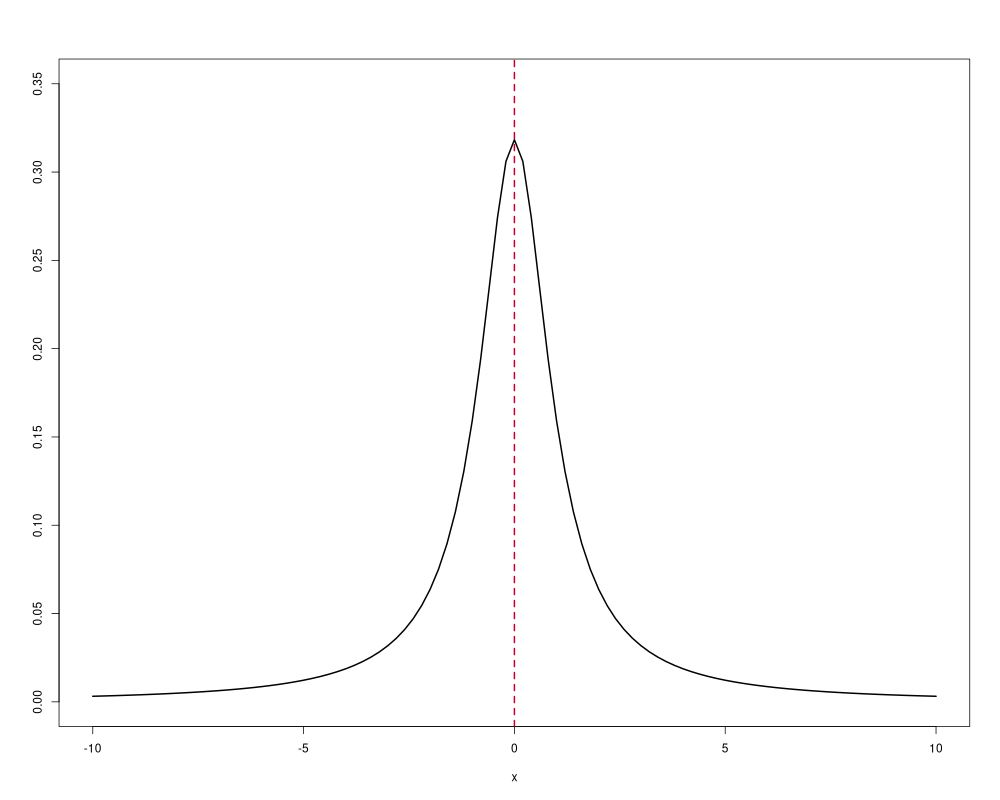
\includegraphics[width=\textwidth]{images/variando_mu_1.png}
            \caption{$\mu = 0$}
        \end{subfigure}%
        ~
        \begin{subfigure}[t]{0.43\textwidth}
            \centering
            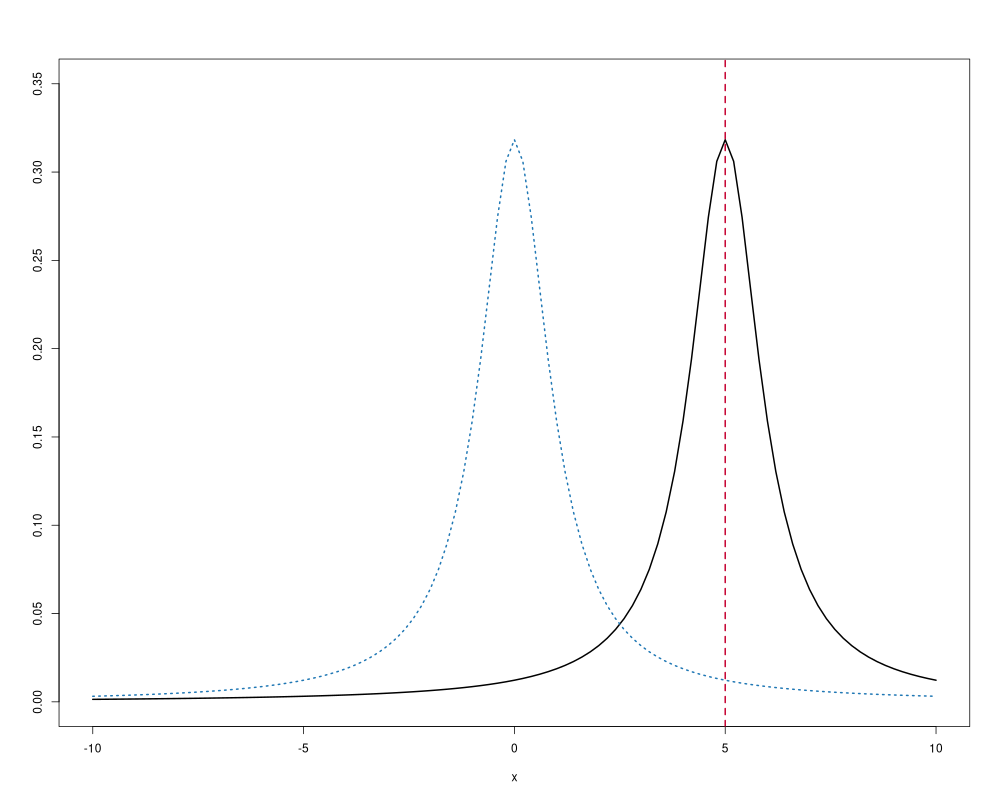
\includegraphics[width=\textwidth]{images/variando_mu_2.png}
            \caption{$\mu = 5$}
        \end{subfigure}%
        \caption{Forma da distribuição para diferentes valores de $\mu$.}
    \end{figure}

    

\end{frame}

\begin{frame}
    \frametitle{Variando $\sigma$}
    
    \begin{figure}[!ht]
        \centering
        \begin{subfigure}[t]{0.43\textwidth}
            \centering
            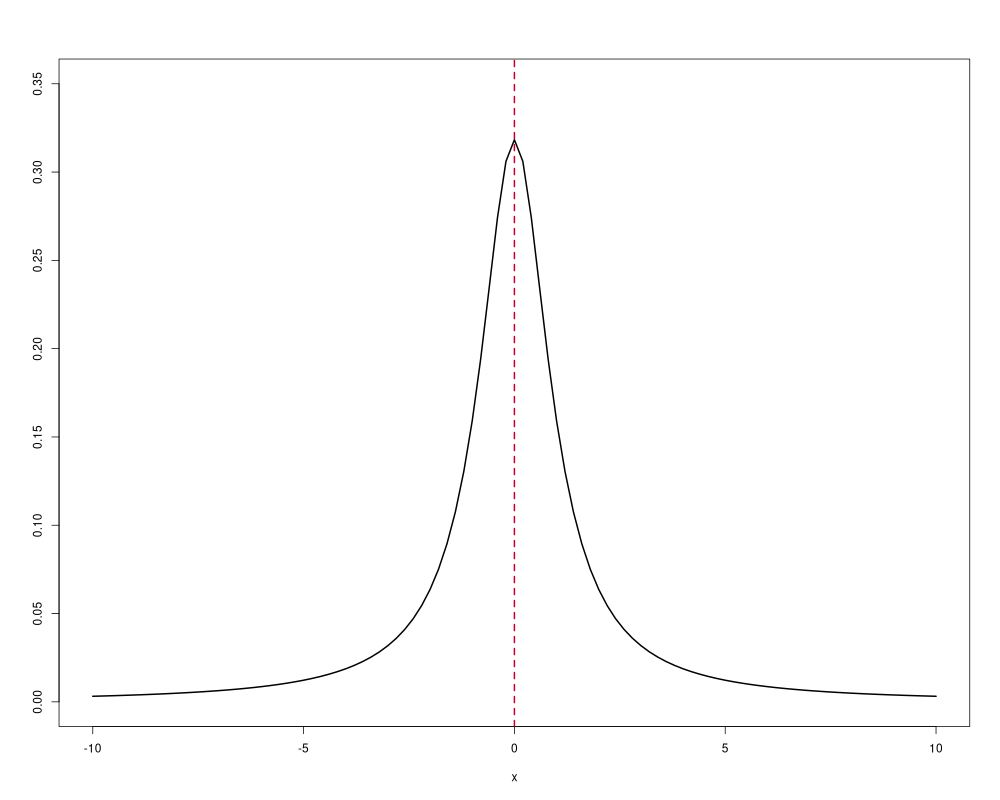
\includegraphics[width=\textwidth]{images/variando_sigma_1.png}
            \caption{$\sigma = 1$}
        \end{subfigure}%
        ~
        \begin{subfigure}[t]{0.43\textwidth}
            \centering
            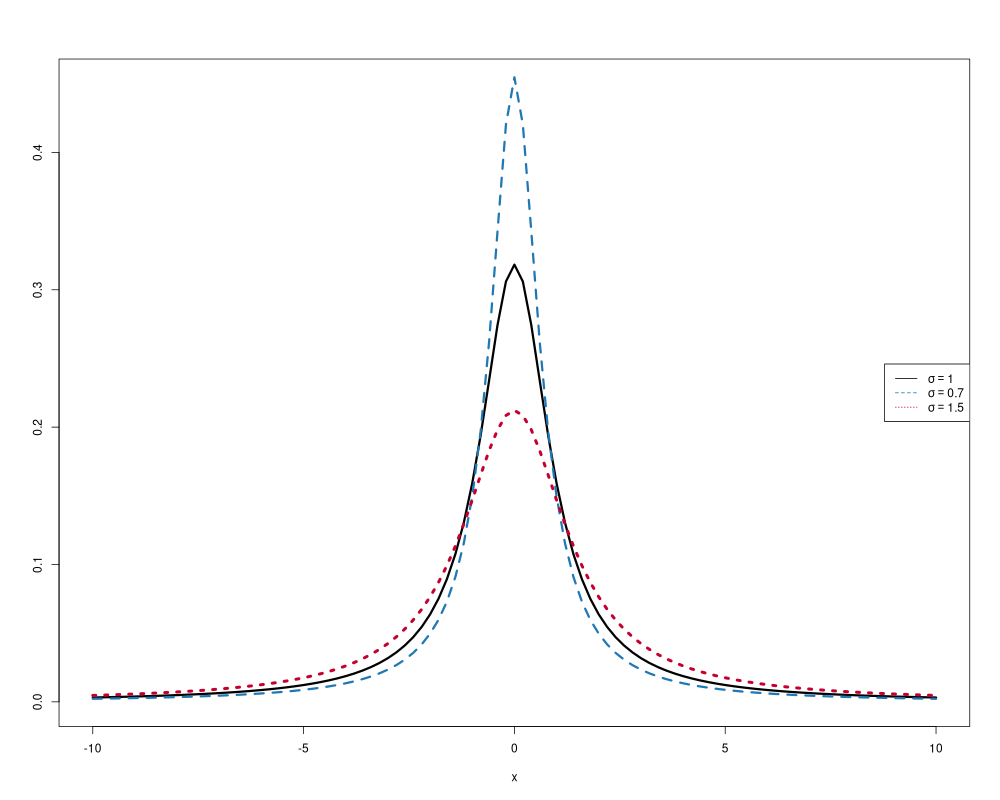
\includegraphics[width=\textwidth]{images/variando_sigma_2.png}
            \caption{$\sigma = 0.7, \,\, 1.5$}
        \end{subfigure}%
        \caption{Forma da distribuição para diferentes valores de $\sigma$.}
    \end{figure} 

\end{frame}

\begin{frame}
    \frametitle{Variando $\nu$}
    
    \begin{figure}[!ht]
        \centering
        \begin{subfigure}[t]{0.43\textwidth}
            \centering
            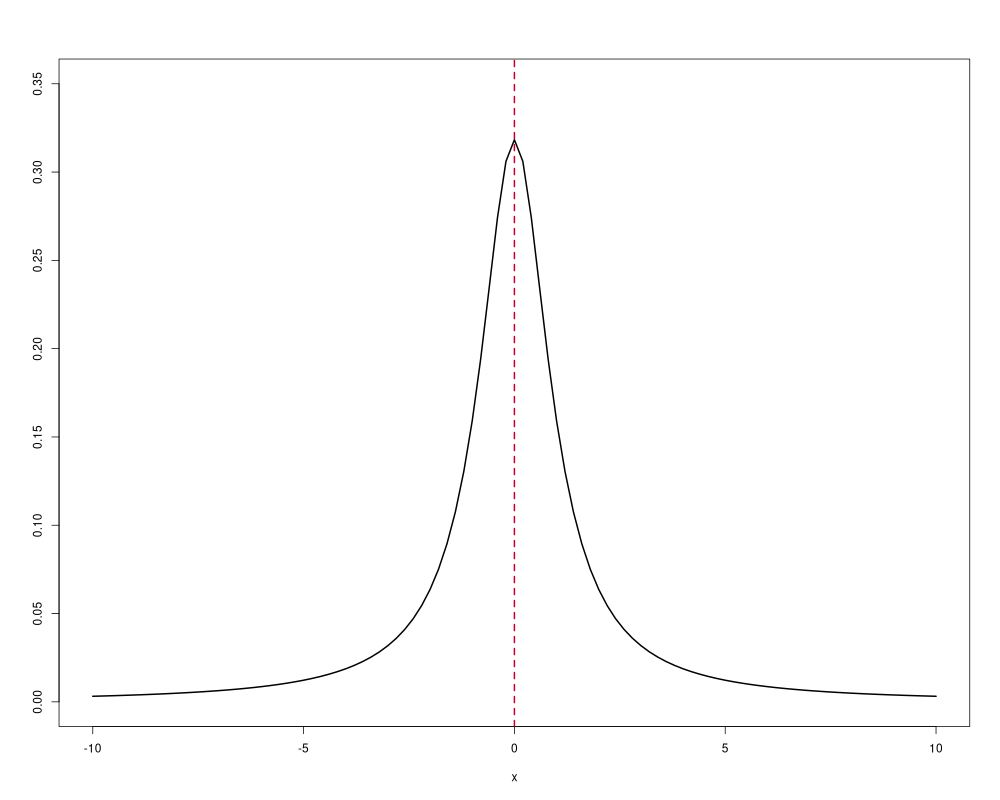
\includegraphics[width=\textwidth]{images/variando_mu_1.png}
            \caption{$\nu = 1$}
        \end{subfigure}%
        ~
        \begin{subfigure}[t]{0.43\textwidth}
            \centering
            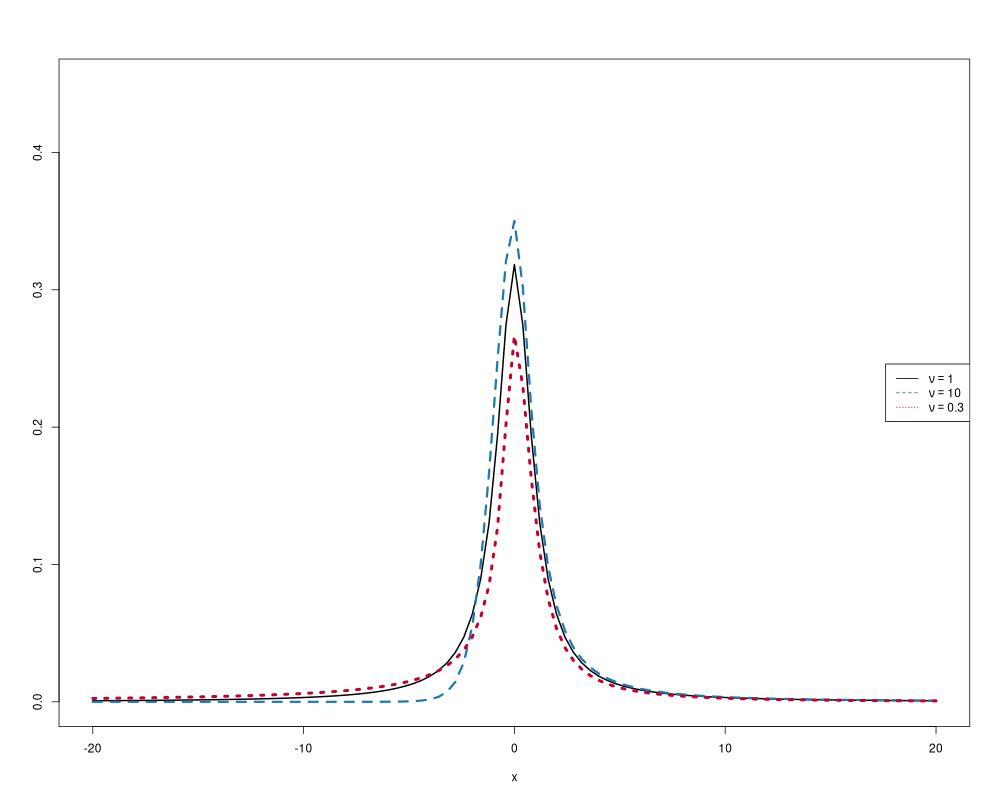
\includegraphics[width=\textwidth]{images/variando_nu_2.png}
            \caption{$\nu = 0.3, \,\, 30$}
        \end{subfigure}%
        \caption{Forma da distribuição para diferentes valores de $\nu$.}
    \end{figure} 

\end{frame}

\begin{frame}
    \frametitle{Variando $\tau$}

    \begin{figure}[!ht]
        \centering
        \begin{subfigure}[t]{0.43\textwidth}
            \centering
            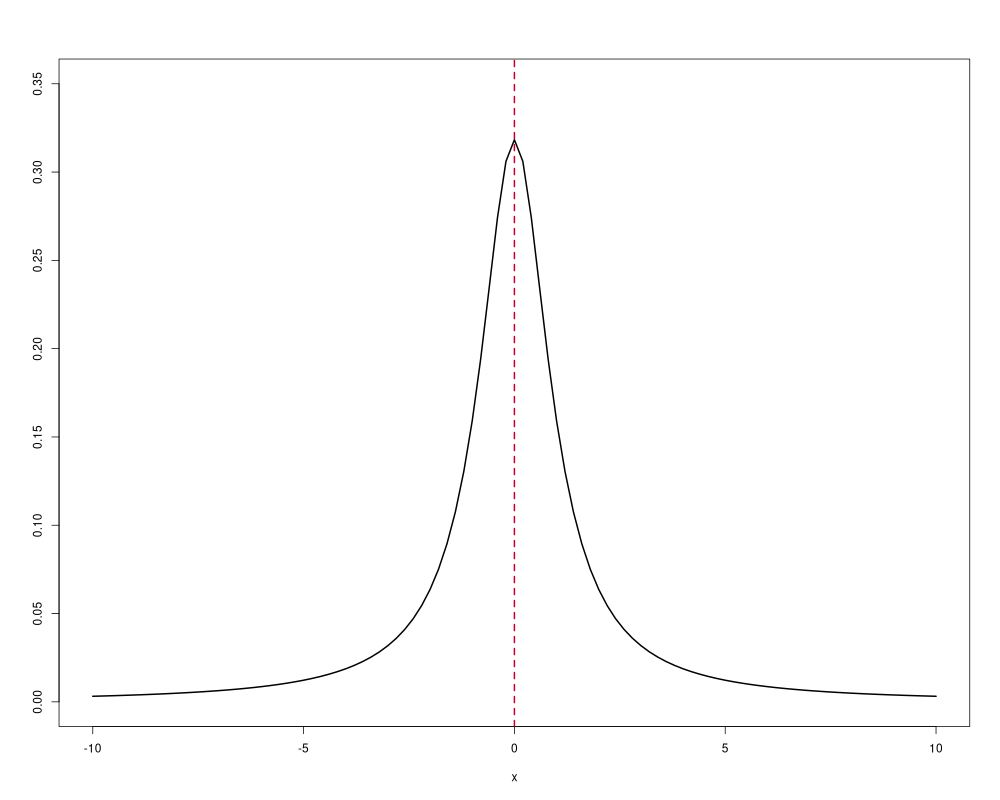
\includegraphics[width=\textwidth]{images/variando_mu_1.png}
            \caption{$\tau = 1$}
        \end{subfigure}%
        ~
        \begin{subfigure}[t]{0.43\textwidth}
            \centering
            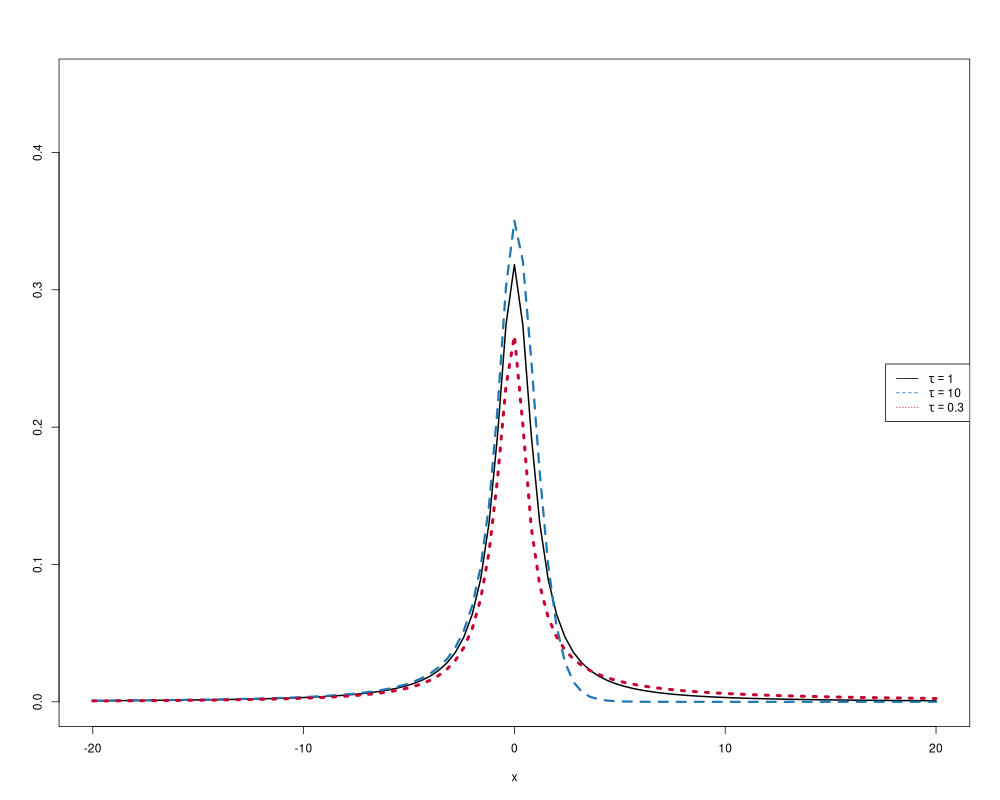
\includegraphics[width=\textwidth]{images/variando_tau_2.png}
            \caption{$\tau = 0.1, \,\, 50$}
        \end{subfigure}%
        \caption{Forma da distribuição para diferentes valores de $\tau$.}
    \end{figure}
\end{frame}

\begin{frame}
    \frametitle{Exemplos}

    \begin{figure}[!ht]
        \centering
        \begin{subfigure}[t]{0.43\textwidth}
            \centering
            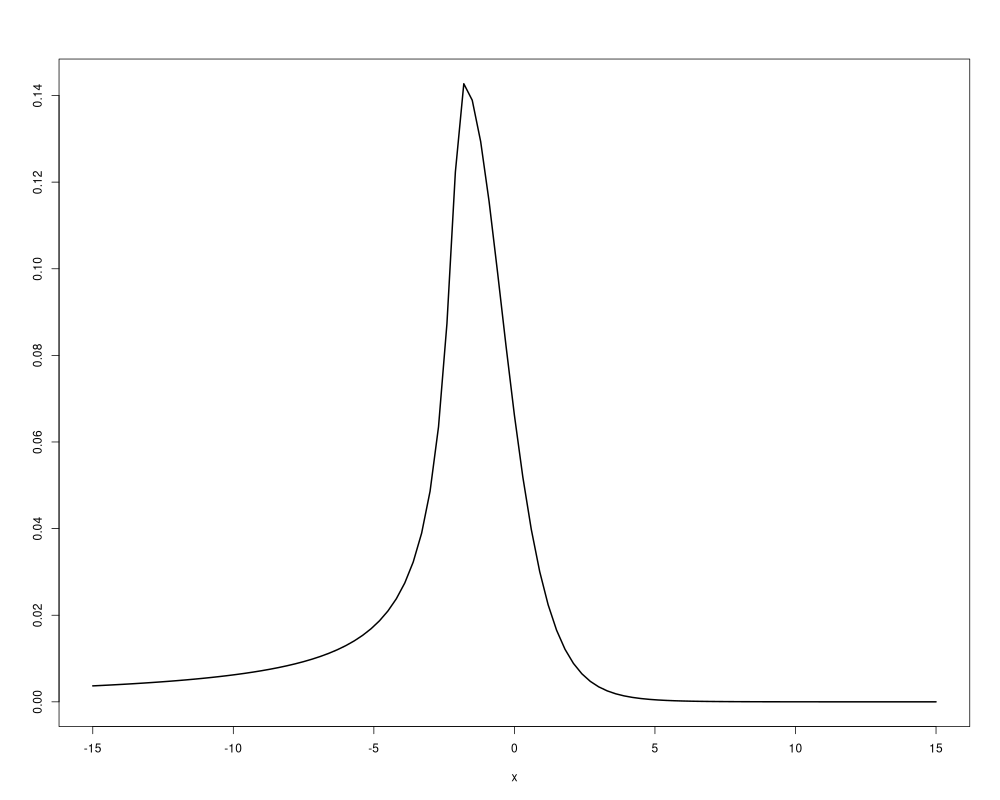
\includegraphics[width=\textwidth]{images/dist_1.png}
            \caption{$\mu = -1.83, \sigma = 1.5, \nu = 0.1, \tau = 7.8$}
        \end{subfigure}%
        ~
        \begin{subfigure}[t]{0.43\textwidth}
            \centering
            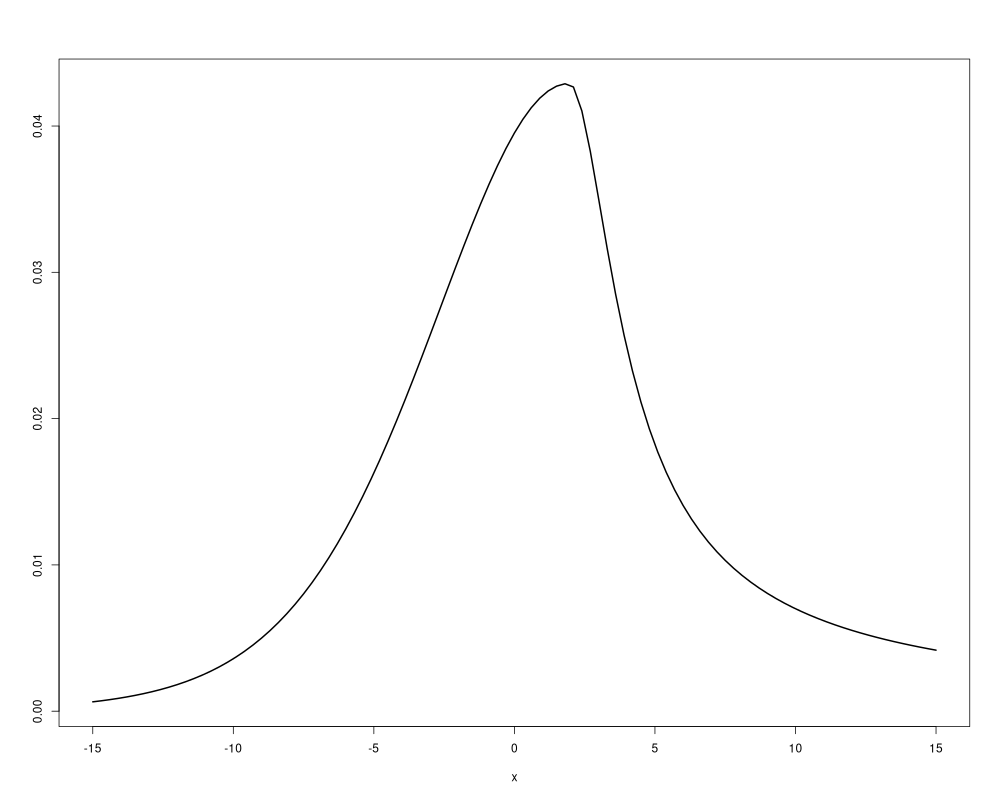
\includegraphics[width=\textwidth]{images/dist_2.png}
            \caption{$\mu = 1.94, \sigma = 5, \nu = 10, \tau = 0.1$}
        \end{subfigure}%
        \caption{Formas da distribuição para diferentes valores dos parâmetros.}
    \end{figure}
\end{frame}

\subsection{Comparando com distribuições mais conhecidas}

\begin{frame}
    \frametitle{Comparando com distribuições mais conhecidas}

   \begin{figure}[!ht]
        \centering
        \begin{subfigure}[t]{0.43\textwidth}
            \centering
            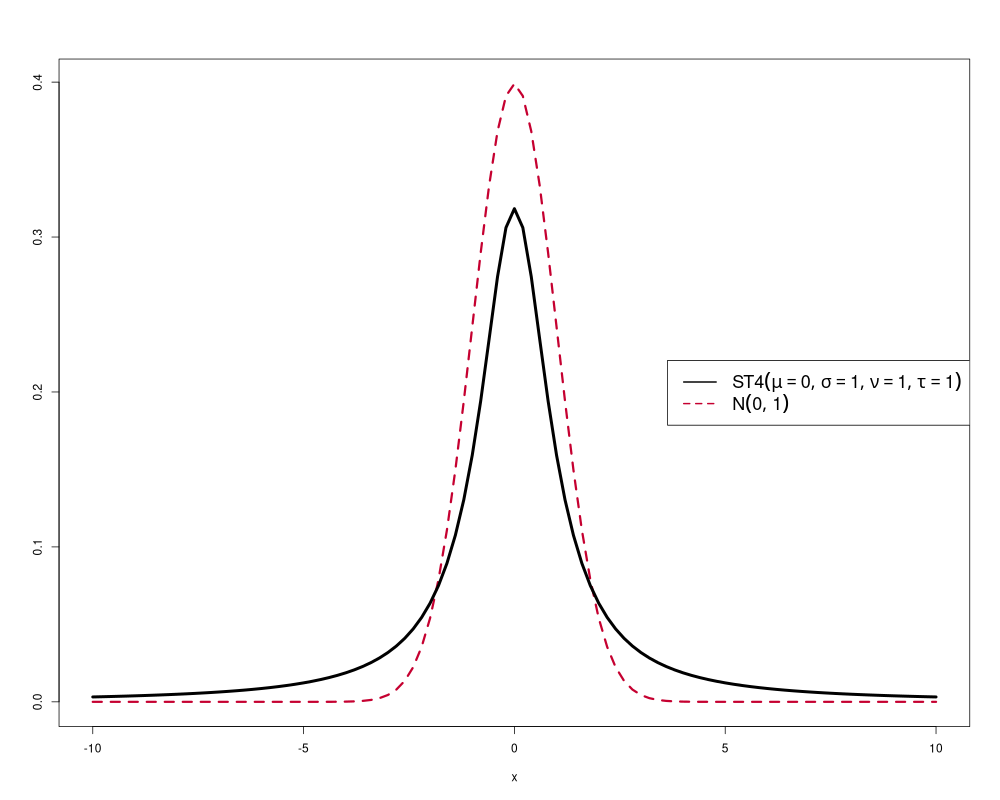
\includegraphics[width=\textwidth]{images/comparando_dists_1.png}
            \caption{}
        \end{subfigure}%
        ~
        \pause
        \begin{subfigure}[t]{0.43\textwidth}
            \centering
            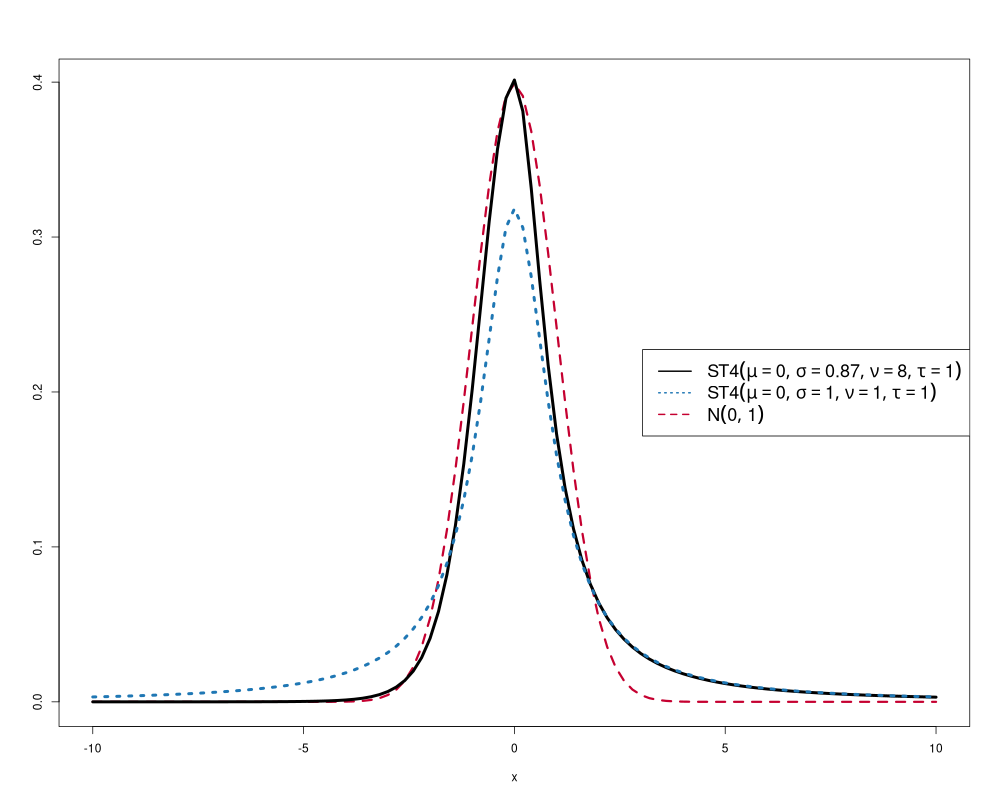
\includegraphics[width=\textwidth]{images/comparando_dists_2.png}
            \caption{}
        \end{subfigure}%
        \caption{}
    \end{figure} 

\end{frame}

\begin{frame}
    \frametitle{Comparando com distribuições mais conhecidas}

   \begin{figure}[!ht]
        \centering
        \begin{subfigure}[t]{0.43\textwidth}
            \centering
            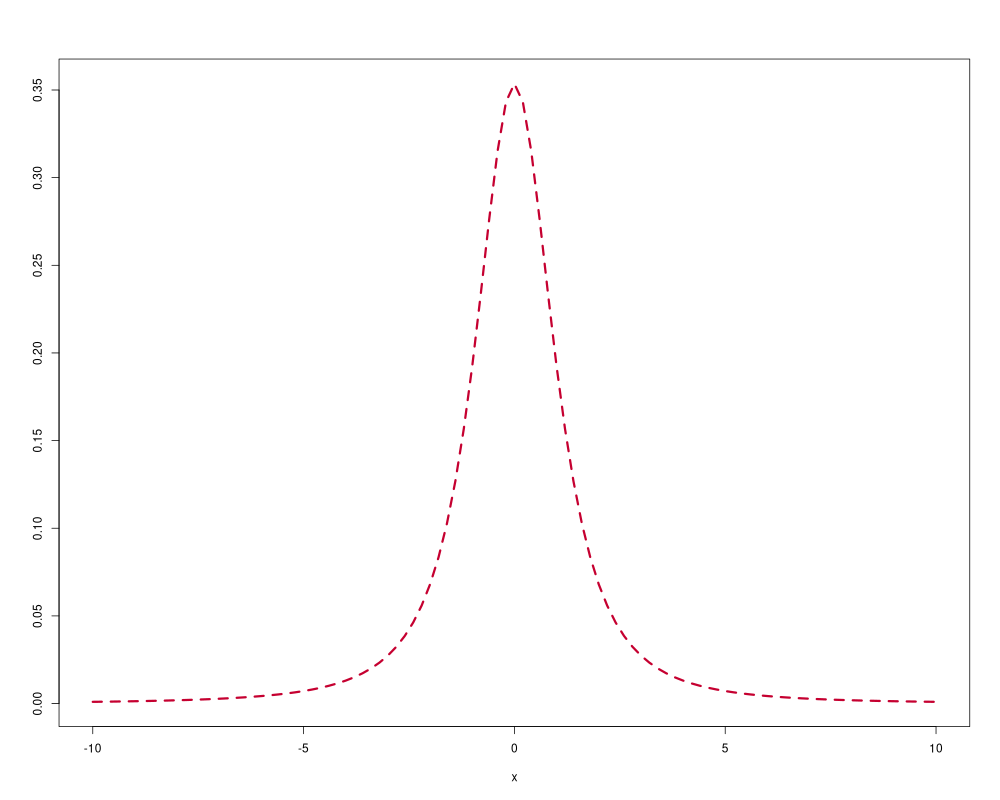
\includegraphics[width=\textwidth]{images/comparando_dists_3.png}
            \caption{}
        \end{subfigure}%
        ~
        \pause
        \begin{subfigure}[t]{0.43\textwidth}
            \centering
            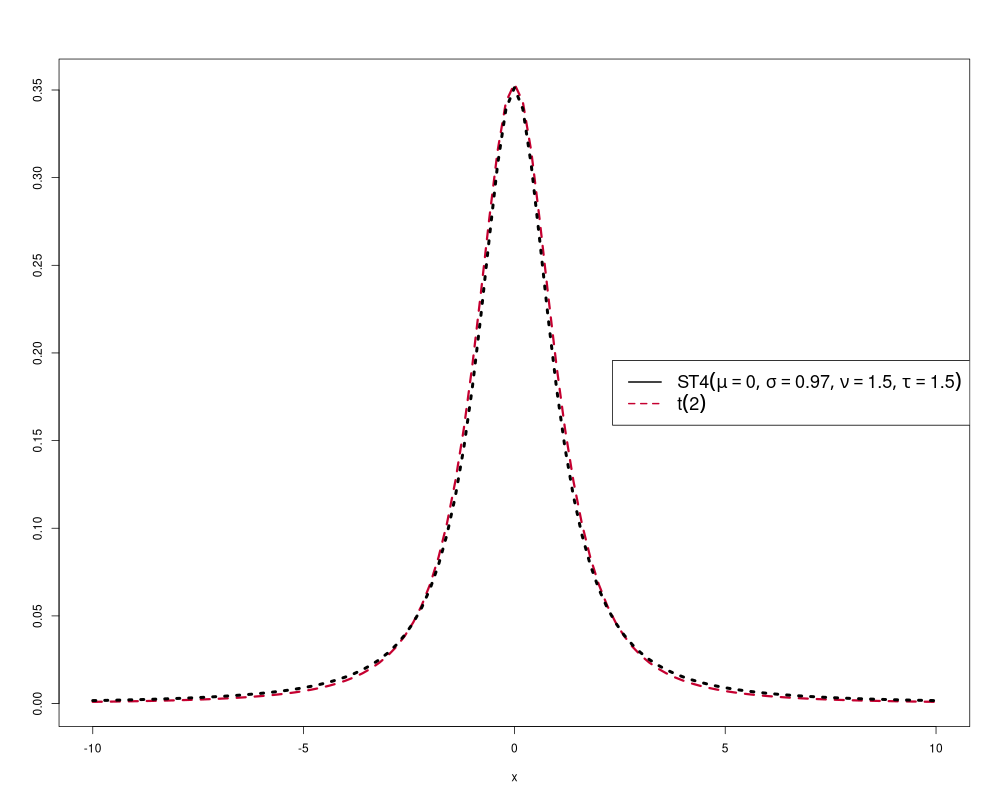
\includegraphics[width=\textwidth]{images/comparando_dists_4.png}
            \caption{}
        \end{subfigure}%
        \caption{}
    \end{figure} 

\end{frame}

\section{Exemplo Prático}

\subsection{Metodologia}

\begin{frame}
    \frametitle{Exemplo Prático -- Metodologia}
    \begin{itemize}
        \item Além do estudo \citetitle{campos2010ajuste} de \textcite{campos2010ajuste} previamente apresentado, mais uma aplicação na área da biologia é dada por \citetitle{rossi2014modelagem} de \textcite{rossi2014modelagem};
        \pause
        \item O objetivo do trabalho foi avaliar o ajuste de diferentes modelos não-lineares a dados de peso corporal de codornas assumindo diferentes distribuições para o erro sob o ponto de vista Bayesiano;
    \end{itemize}

\end{frame}

\begin{frame}
    \frametitle{Exemplo Prático -- Metodologia}

    \begin{itemize}
        \item O experimento utilizou $1.831$ codornas de corte (\textit{Coturnix coturnix japonica}), sendo constituido de $903$ fêmeas e $928$ machos.
        \pause
        \item Os animais foram pesados semanalmente, formando um banco de dados para peso corporal (em gramas) ao nascimento, $7$, $14$, $21$, $28$ e $35$ dias de idade.
    \end{itemize}

\end{frame}

\begin{frame}
    \frametitle{Exemplo Prático -- Metodologia}

    \begin{itemize}
        \item O estudo foi constituido das seguintes etapas:
           \begin{enumerate}
                \item Consistiu em considerar alguns modelos não-lineares mais utilizados para descrever curvas de crescimento de aves em diferentes formas parametrizadas, assumindo-se distribuição normal para os erros e selecionar aquele que melhor se ajusta aos dados por meio da inferência Bayesiana.
                \pause
                \item Consideram-se distribuições alternativas à normal para o erro, sendo elas a distribuição $t$, a skew-normal e skew-$t$. 
            \end{enumerate}
    \end{itemize}

\end{frame}

\subsection{Resultados}

\begin{frame}
    \frametitle{Exemplo Prático -- Resultados}

    \begin{itemize}
        \item Os autores concluem tanto em um estudo simulado, quanto em uma aplicação a dados reais, que ao utilizar a curva de crescimento descrita por
            \begin{equation*}
                f(x) = \beta_1 (1 - \beta_2 e^{\beta_3 x} )^3
            \end{equation*}
            o modelo skew-$t$ para os erros é o mais adequado por apresentar maior probabilidade de cobertura dos intervalos de credibilidade para os verdadeiros valores dos parâmetros e menor DIC (\textit{Deviance Information Criterion}).
    \end{itemize}

\end{frame}

\begin{frame}
    \frametitle{Exemplo Prático -- Resultados}

    \vspace{-0.5cm}

    \begin{table}
        \centering
        \footnotesize
        \resizebox{\linewidth}{!} - P_{97.5\%}$ & & Média (dp) & $P_{2.5\%} - P_{97.5\%}$ \\
                                      \midrule
                1 & 9,50$^{a}$ (0,031) & 9,45 - 9,57 & & 9,58$^{a}$ (0,033) & 9,52 - 9,65 \\
                7 & 29,66$^{a}$ (0,164) & 29,34 - 29,98 & & 29,81$^{a}$ (0,169) & 29,47 - 30,14 \\
                14 & 76,56$^{a}$ (0,314) & 75,95 - 77,18 & & 76,88$^{a}$ (0,365) & 76,17 - 77,60 \\
                21 & 139,00$^{b}$ (0,472) & 138,10 - 139,90 & & 145,50$^{a}$ (0,592) & 140,40 - 142,70 \\
                28 & 192,30$^{b}$ (0,553) & 191,20 - 193,40 & & 197,50$^{a}$ (0,656) & 196,20 - 198,80 \\
                35 & 225,70$^{b}$ (0,639) & 224,40 - 226,90 & & 235,90$^{a}$ (0,724) & 234,50 - 237,40 \\
                \bottomrule
            \end{tabular}
        }
        \vspace{0.3cm}
        \footnotesize
        \centering
        \begin{minipage}{\linewidth}
            $dp$= \textit{desvio-padrão da média}; $P_{2.5\%} - P_{97.5\%}$ = \textit{intervalo com} $95\%$ \textit{de credibilidade;} \\
            $^{a,b}$ \textit{Letras distintas na linha, indicam diferenças significativas entre as médias dos pesos (g), por meio de comparações Bayesianas em nível de 95\% de credibilidade.} \\
            \textbf{Fonte}: \textcite{rossi2014modelagem}.
        \end{minipage}
    \end{table}

\end{frame}

\begin{frame}
    \frametitle{Exemplo Prático -- Resultados}
    \small
    A segunda etapa da análise indicou que assumindo erros skew-normais e skew-$t$ para os machos e fêmeas, respectivamente, obtemos os melhores ajustes para os dados de pesos corporais de codornas.

    \begin{figure}[!ht]
        \centering
        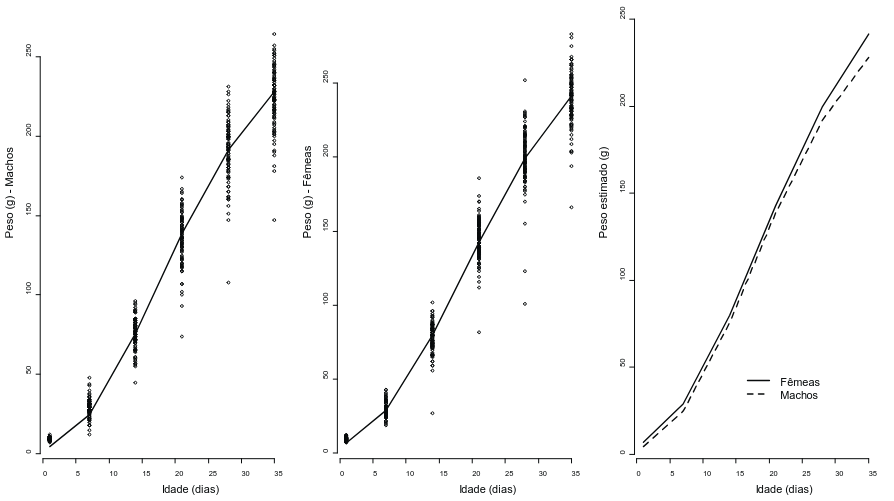
\includegraphics[width=0.53\linewidth]{images/peso_codornas.png}
        \scriptsize
        \caption{\scriptsize Curvas de \textit{Gompertz - $f_2$} ajustadas a dados de peso (g), por meio do procedimento $P_1$, com erros skew-normais e skew-$t$, respectivamente, para machos e fêmeas.}
        \label{fig:peso_codornas}
        \vspace{-0.3cm}
        \begin{minipage}{\linewidth}
            \textbf{Fonte}: \textcite{rossi2014modelagem}.
        \end{minipage}
    \end{figure}

\end{frame}

\subsection{Conclusões}

\begin{frame}
    \frametitle{Exemplo Prático -- Conclusões}

    O modelo não-linear de Gomperts na forma parametrizada $f_2$, com erros skew-normais e skew-$t$, respectivamente, para machos e fêmeas, por meio do procedimento proposto por \textcite{de2009bayesian}, foi o que melor ajustou os dados de pesos corporal das codornas. 
    

\end{frame}

\section{Conclusão}

\begin{frame}
    \frametitle{Conclusão}

    \begin{itemize}
        \item A distribuição pode ser utilizada quando a distribuição dos dados assume valores na reta real e possui natureza assimétrica com caudas pesadas.
        \pause
        \item As principais vantages se resuem a grande capacidade de adaptabilidade da distribuição, podemos alterar o peso de cada uma de suas caudas, podemos alterar a sua curtose e sua locação, viabilizando uma maior aderência aos dados.
        \pause
        \item A distribuição é limitada quando se tratam de dados que assumem valores somente positivos ou negativos.
        \pause
        \item A forma da distribuição pode ser mostrada graficamente por meio do comando \texttt{demo.ST4()}, em que, de forma interativa, todos os parâmetros podem ser ajustados.
        \pause
        \item Um método alternativo para mostrar a função densidade de probabilidade é utilizar a função \texttt{pdf.plot(family = ST4, mu = c(0, 3), sigma = c(1, 5), nu = c(1, 0.5), tau = 1)}
    \end{itemize}

\end{frame}

\section{Referências}

\begin{frame}
    \frametitle{Referências}

    \printbibliography{}

\end{frame}

\end{document}
